\documentclass[a4paper]{article}
\usepackage{cmap}
\usepackage{mathtext}
\usepackage{amssymb}
\usepackage{amsmath}
\usepackage[russian]{babel}
\usepackage{indentfirst}
\usepackage[pdftex]{graphicx}
\usepackage{multirow}
\usepackage{siunitx}
\usepackage[left=2cm,right=2cm,top=2cm,bottom=2cm]{geometry}
\usepackage{fancyhdr}
\pagestyle{fancy}
\newcommand{\rref}[1]{(\ref{#1})}
\newcommand{\Equip}[3]{{\bf #1:} $\Delta = \pm #2$ \si{#3}

}
\newcommand{\equip}[1]{{\bf #1}

}
\newcommand{\labname}{Закон Кюри-Вейсса.} 	% название пиши здесь
\newcommand{\labnum}{3.4.2.}										% номер вводи здесь
\fancyfoot{}
\fancyhead[RE, RO]{\thepage}
\fancyhead[LE, LO]{Лабораторная работа \labnum \space \labname}
\title{Лабораторная работа \labnum \space \labname} % Название работы здесь
\author{Иван Сладков}
\begin{document}
\maketitle
\thispagestyle{empty}
\section{Аннотация}
В данной работе проводится исследование зависимости магнитной восприимчивости гадолиния, который является ферромагнетиком, от температуры. Исследование приведено для температур от 14 до 40 \si{\degreeCelsius}. На основании этой зависимости вычисляется точка Кюри гадолиния.
\section{Теоретические сведения}
Одной из основных макроскопических характеристик веществ, которая используется для описания их магнитных свойств, является вектор намагниченности $\mathbf{M}$ — суммарный магнитный момент единичного
объёма вещества. В ряде веществ между намагниченностью $\mathbf{M}$ и напряжённостью магнитного поля $\mathbf{H}$ имеет место линейная зависимость:
где скалярная величина $\chi$ — магнитная восприимчивость единичного
объёма вещества. Вещества с отрицательной магнитной восприимчивостью $(\chi < 0)$ называют диамагнетиками, а вещества с $(\chi >0)$ принадлежат к классу парамагнетиков.

Кроме диа- и парамагнетиков ($\chi \le 10^{-3}$) существуют также ферромагнетики, для которых $\chi \ge 10^{4}$. Причём зависимость $\mathbf{M(H))}$ в таких веществах нелинейна. 

Магнитные и другие физические свойства ферромагнетиков зависят от температуры. Намагниченность насыщения $M_s$ (равная максимальной намагниченности при данной температуре) имеет максимум при $T=0$ и монотонно убывает до $0$ при $T=\Theta$ -- температуре Кюри. Поведение ферромагнетика при больших температурах описывается законом Кюри-Вейсса:
\begin{equation}
	\chi = \frac{C}{T-\Theta_p},
	\label{a}
\end{equation}
где $\Theta_p$ -- парамагнитная температура Кюри.
\subsection{Расчётные формулы}
Магнитная восприимчивость определяется по формуле:
\begin{equation}
	(L-L_0)\sim \chi,
\end{equation}
где $L$ -- самоиндукция катушки с образцом, а $L_0$ -- без образца. Тогда из 
\begin{align}
	\tau = 2 \pi \sqrt{L C}, \\
	\tau_0 = 2 \pi \sqrt{L_0 C}
\end{align}
следует:
\begin{align}
	(L-L_0)\sim (\tau^2 - \tau_0^2), \\
	\chi \sim (\tau^2 - \tau_0^2).
	\label{b}
\end{align}

Из \rref{a} и \rref{b}, окончательно: 
\begin{equation}
	\frac{1}{\chi}\sim \frac{1}{\tau^2 - \tau^2_0}
\end{equation}
\section{Оборудование и инструментальные погрешности}

%{\bf : } $\Delta = \pm  $ ед
Оборудование, используемое в работе, представлено на рис. \ref{fig:set}. Исследуемый образец находится внутри индуктивности в колбе с трансформаторным маслом, температура которого поддерживается термостатом. Катушка является частью LC-контура, частота которого фиксируется частотомером.

\equip{Автогенератор }
\Equip{Цифровой вольтметр}{1*10^{-5}}{\volt}
\Equip{Частотомер}{1*10^{-5}}{\volt}
\Equip{Термостат}{0.1}{\degreeCelsius}
{\bf LC-контур: }$\tau_0 = 6.9092 $ \si{\micro \second}

\begin{figure}
	\centering
	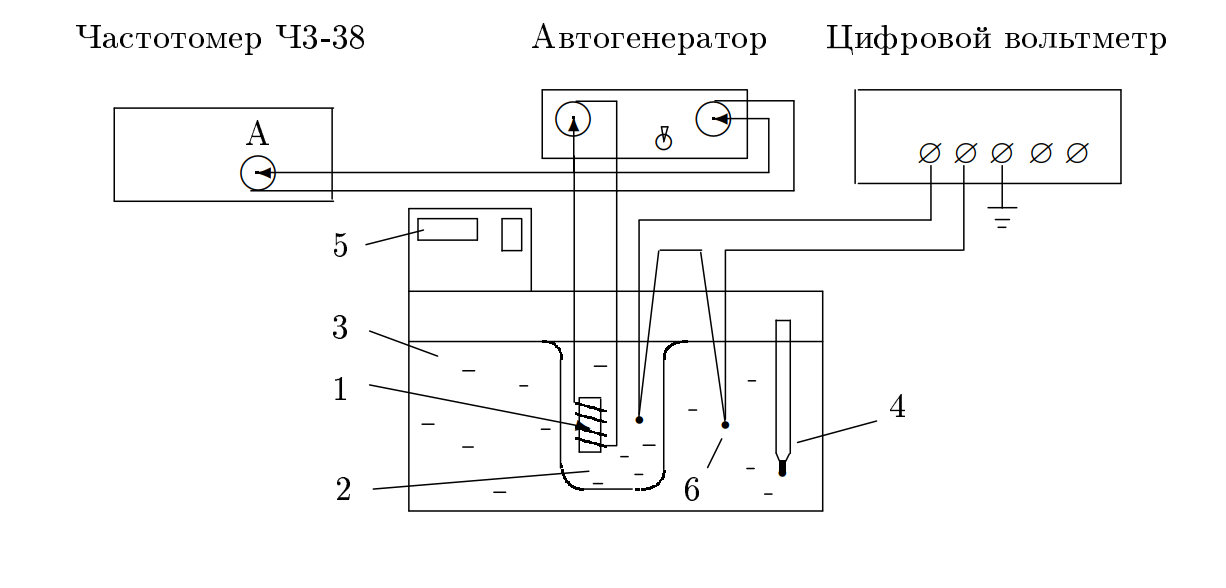
\includegraphics[width=1\linewidth]{Screenshot_1}
	\caption{Экспериментальная установка}
	\label{fig:set}
\end{figure}

\section{Результаты измерений и обработка данных}

Напряжение на вольтметре при $\Delta T
= 0.5$ \si{\degreeCelsius} равно $20$ \si{\micro \volt}.

Исходные результаты измерений в табл. 1.

\begin{table}[]
	\centering
	\label{tab}
	\begin{tabular}{|l|l|l|l|}
		\hline
		\textbf{Температура термостата, \si{\degreeCelsius}} & \textbf{Напряжение, \si{\volt}} & \textbf{Период, \si{\micro \second}} & \textbf{Температура жидкости, \si{\degreeCelsius}} \\ \hline
		14.1                                                 & -15                                          & 7.92                                 & 13.7                                               \\ \hline
		16.1                                                 & -15                                          & 7.855                                & 15.7                                               \\ \hline
		18.1                                                 & -15                                          & 7.744                                & 17.7                                               \\ \hline
		20.1                                                 & -15                                          & 7.56                                 & 19.7                                               \\ \hline
		22.1                                                 & -13                                          & 7.343                                & 21.8                                               \\ \hline
		24.1                                                 & -12                                          & 7.194                                & 23.8                                               \\ \hline
		26.1                                                 & -13                                          & 7.123                                & 25.8                                               \\ \hline
		28.1                                                 & -15                                          & 7.085                                & 27.7                                               \\ \hline
		30.1                                                 & -17                                          & 7.058                                & 29.7                                               \\ \hline
		32.1                                                 & -18                                          & 7.04                                 & 31.7                                               \\ \hline
		34.1                                                 & -18                                          & 7.026                                & 33.7                                               \\ \hline
		36.1                                                 & -19                                          & 7.016                                & 35.6                                               \\ \hline
		38.1                                                 & -19                                          & 7.008                                & 37.6                                               \\ \hline
		40.1                                                 & -18                                          & 7.002                                & 39.7                                               \\ \hline
	\end{tabular}
	\caption{Исходные данные}
\end{table}



\subsection{Оценка погрешностей}

\section{Вывод}

\begin{thebibliography}{9}
\bibitem{Siv} Сивухин Д. В. \emph{Общий курс физики. Том 2 Термодинамика и молекулярная физика}, 2003
\end{thebibliography}
\end{document}

